\section{Technologia NFC (Konrad Ossowski)}
NFC (ang. Near Field Communication) to w dosłownym tłumaczeniu komunikacja bliskiego zasięgu. Polega ona na bezprzewodowej technologii krótkiego zasięgu. Tag NFC to pasywne urządzenie NFC, zasilane polem NFC urządzenia, gdy znajduje się ono w zasięgu. Wyróżnia się cztery rodzaje tagów, różnią się od siebie pojemnością i/lub formatem.  Zazwyczaj wymagają odległości 4cm lub mniejszej, aby zainicjować połączenie.  Tagi mogą mieć różną złożoność. Proste znaczniki oferują tylko możliwość odczytu i zapisu, czasem z programowalnym obszarem infromującym, że zawartość jest tylko do odczytu. Bardziej skomplikowane tagi oferują operacje matematyczne i mają sprzęt kryptograficzny do uwierzytelniania. Najbardziej wyrafinowane tagi zawierają środowisko operacyjne, pozwalające na złożone interakcje z kodem wykonującym na tagu.
\paragraph{Zasada działania}\mbox{}\\
NFC opiera się na efekcie indukcji elektromagnetycznej. Gdy znacznik znajdzie się obrębie pola magnetycznego, generowana jest energia elektryczna. Sygnał przepływa między dwiema antenami – w smartfonie i w sprzęcie docelowym (również może to być smartfon). W ten sposób zestabilizowane zostaje połączenie zapewniające komunikację między urządzeniami za pomocą fal radiowych krótkiego zasięgu.
\subsection{Historia NFC}
Pierwsze próby z tą technologią rozpoczęto jeszcze na początku lat 80. W 1983 r. złożono wówczas pierwszy patent związaniu z technologią RFID (ang. Radio-frequency identification), która jest inspiracją dla NFC. Dopiero w 2004 roku została utworzona organizacja mająca na celu rozwój technologii NFC - NFC Forum.
\par
Trzeba było kolejnych lat, by dopiero w 2009 r. zostały opracowane kolejne elementy układanki, która pozwoliła na wygodne korzystanie z NFC. Dopiero siedem lat temu zaczęły działać pierwsze standardy przesyłania zarówno kontaktów czy adresów URL. W tym samym czasie stworzono również sposób na inicjalizację nadajnika Bluetooth. Dzięki temu nie trzeba korzystać z niezbyt wygodnego parowania urządzeń. Zamiast tego wystarczy zbliżyć do siebie czytnik (smartfon) z kartą NFC (głośnik bezprzewodowy) by nawiązać między nimi łączność Bluetooth.
\subsection{NFC na platforie Android}
Funkcja NFC umożliwia udostępnianie niewielkich ładunków danych między tagiem NFC, a urządzeniem z systemem Android lub między dwoma urządzeniami. Dane przechowywane w tagu mogą być również zapisane w różnych formatach, ale wiele interfejsów API systemu Android jest opartych na standardzie NFC Forum o nazwie Ndef. Urządzenia z systemem Android z obsługą NFC realizują jednocześnie trzy główne tryby działania:
\begin{itemize}
\item Tryb czytnika/zapisywacza - umożliwia urządzeniu NFC odczytywanie i/lub zapisywanie pasywnych tagów NFC i naklejek.
\item Tryb peer-to-peer - umożliwia urządzeniu NFC wymianę danych z innym urządzeniem NFC. Korzysta z niego funkcja Android Beam.
\item Tryb emulacji kart - umożliwia urządzeniu NFC działać jak karta NFC. Dostęp do emulowanej karty NFC można uzyskać za pomocą zewnętrznego czytnika np. terminalu płatniczego NFC.
\end{itemize}
 Funkcja Android Beam umożliwia urządzeniu przesyłanie wiadomości NDEF na inne urządzenie poprzez fizyczne dotykanie urządzeń. Ta interakcja zapewnia łatwiejszy sposób wysyłania danych niż inne technologie bezprzewodowe, takie jak Bluetooth, ponieważ w przypadku NFC nie jest wymagane ręczne wykrywanie urządzeń ani parowanie. Połączenie zostanie automatycznie uruchomione, gdy dwa urządzenia znajdą się w zasięgu.
\subsubsection{NfcAdapter}
Reprezentuje lokalny moduł NFC. Posiada trzy stałe określające akcję dla Intencji:
\begin{itemize}
    \item \textit{ACTION\_TAG\_DISCOVERED} - dowolny tag NFC został wykryty
    \item \textit{ACTION\_NDEF\_DISCOVERED} - został wykryty tag z danymi NDEF
    \item \textit{ACTION\_TECH\_DISCOVERED} - został wykryty tag, którego technologia została zarejestrowana w jakieś Aktywności
\end{itemize}
Tworzenie nowego obiektu zawierającego strukturę NfcAdapter sprowadza się do wywołania statyczej metody tej klasy \textit{getDefaultAdapter(context)}. Poniżej przedstawiony jest konstruktor zaimplementowanej przez nas klasy NfcService. 
\begin{lstlisting}[language=Java]
public NfcService(Context context){
        this.context = context;
        this.nfcAdapter = NfcAdapter.getDefaultAdapter(context);
}
\end{lstlisting}
W parametrze \textit{context} przekazywany jest obiekt Aktywności, która korzysta z NFC. Dodatkowo, aby nasza Aktywność miała pierwszeństwo do obsłużenia wykrytego tagu, gdy jest na pierwszym planie, musimy nadpisać jej metodę onResume(). W ciele tej metody musi występować wywołanie funkcji klasy NfcAdapter \textit{enableForegroundDispatch (Activity activity, PendingIntent intent, IntentFilter[] filters, String[][] techLists)}. Jeśli został podany parametr \textit{filters}, jest ona używany do dopasowania Intencji wysyłanych zarówno dla \textit{ACTION\_NDEF\_DISCOVERED}, jak i \textit{ACTION\_TAG\_DISCOVERED}. Ponieważ \textit{ACTION\_TECH\_DISCOVERED} opiera się na metadanych zawartych w tagu, jego dopasowanie jest obsługiwane przez osobną listę zarejestrowanych technologii w parametrze \textit{techLists}. Jeśli parametry \textit{filters} i \textit{techList} będą \textit{null} to wszystkie wykryte znaczniki zostanę przekazane do Aktywności na pierwszym planie. W naszej klasie klasie NfcService, zostało to zrealizowane w postaci publicznej metody, która może zostać wywołana z poziomu Aktywności, gdzie został utworzony obiekt klasy NfcService.
\begin{lstlisting}[language=Java]
public void enableForegroundDispatchSystem(){
    Intent intent = new Intent(context, context.getClass());
    intent.addFlags(Intent.FLAG_RECEIVER_REPLACE_PENDING);
    Intent[] intentArray = new Intent[]{intent};
    PendingIntent pending = PendingIntent.getActivities(context, 0, intentArray, 0);
    IntentFilter[] filters = new IntentFilter[] {};
    nfcAdapter.enableForegroundDispatch((Activity)context, pending, filters, null);
}
\end{lstlisting}
Gdy Aktywność obługująca wykryte tagi NFC zniknie z pierwszego planu, należy niezwłocznie wyłączyć jej tę możliwość. Najlepiej zrobić to w nadpisanej metodzie \textit{onPause()} Aktywności korzystającej z NFC. 
\begin{lstlisting}[language=Java]
public void disableForegroundDispatchSystem(){
        nfcAdapter.disableForegroundDispatch((Activity)context);
}
\end{lstlisting}
\subsubsection{Znacznik}
Znacznik (ang. Tag) jest to niezmienny obiekt rezprezentujący stan znacznika NFC w momencie wykrycia. Może być używany jako uchwyt, aby wykonywać bardziej zaawansowane operacje. Nowy obiekt Znacznika jest tworzony za każdym razem, gdy moduł NFC go wykryje. Nie ma znaczenia czy jest to fizycznie ten sam znacznik. Uzyskanie obiektu Znacznika jest możliwe poprzez wyciągnięcie go z obiektu Intencji przekazanego do Aktywności pierwszego planu. Dlatego tak ważne jest uruchamianie metody enableForegroundDispatch(), w metodzie onResume() Aktywności. 
\begin{lstlisting}[language=Java]
public boolean setNfcTag(Intent intent) {
        if(intent.hasExtra(NfcAdapter.EXTRA_TAG)){
            tag = getTag(intent);
            return true;
        }
        return false;
}
private Tag getTag(Intent intent) {
        return intent.getParcelableExtra(NfcAdapter.EXTRA_TAG);
}
\end{lstlisting}
Metoda \textit{setNfcTag()} jest wywoływana w nadpisanej metodzie \textit{onNewIntent()} Aktywności, która obsługuje żądanie NFC.
\subsubsection{Zapis i odczyt danych z użyciem tagu NFC}

Ndef (ang. NFC Data Exchenge Format) to lekki format binarny, używany do enkapsulacji wpisanych danych. Jest określony przez NFC Forum do transmisji i przechowywania danych za pomocą NFC. Obiekt tej klasy uzyskuje się za pomocą statycznej metody klasy Ndef \textit{get(Tag tag)}. Zawiera w sobie Wiadomości (ang. NdefMessages) i Rekordy (ang. NdefRecords). Rekordy zawierają w sobie dane, może to być nośnik MIME, URI lub niestandardowe dane aplikacji. Natomiast Wiadomości są zbiorem Rekordów.
\paragraph{Zapis}\mbox{}\\
Zapis danych do tagu polega na poprawnym przygotowaniu Rekordu Ndef. Stworzeniu na jego podstawie Wiadomości Ndef, a następnie nadpisaniu poprzedniej Wiadomości Ndef w znaczniku (o ile znacznik nie jest tylko do odczytu).
\begin{lstlisting}[language=Java]
public boolean writeToNfcTag(String content){
        return writeNdefMessage(content);
}

private NdefMessage createNdefMessage(String content){
    NdefRecord record = NdefRecord.createTextRecord(null, content);
    return new NdefMessage(record);
}

private boolean writeNdefMessage( String content){
    try{
        if(tag == null){
            return false;
        }
        else{
            Ndef ndef = Ndef.get(tag);
            NdefMessage mess = createNdefMessage(content);
            if(ndef == null){
                return false;
            }
            else{
                ndef.connect();
                if(!ndef.isWritable()){
                    ndef.close();
                    return false;
                }
                ndef.writeNdefMessage(mess);
                ndef.close();
                return true;
            }
        }
    }
    catch(Exception e){
        return false;
    }
}
\end{lstlisting}
Efektem graficznym tego fragmentu jest następująca Aktywność. Wyświetlony Toast został wywołany po zbliżeniu znacznika do smartfonu i poprawnym zapisie danych do niego.
\begin{figure}[H]
    \centering
    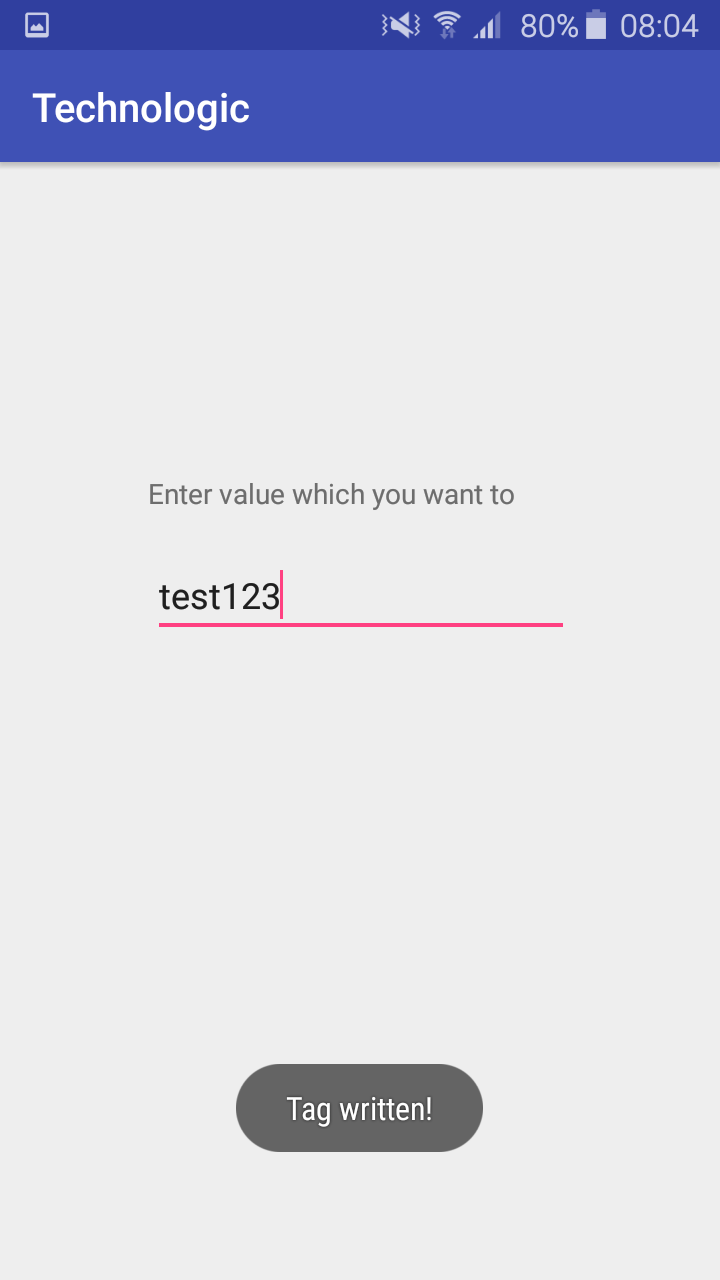
\includegraphics[scale=0.22]{imgs/write.png}
    \caption{Aktywność do zapisywania danych do tagu NFC}
\end{figure}
\paragraph{Odczyt}\mbox{}\\
Odczyt danych Ndef z tagu NFC jest obsługiwany za pomocą systemu rozsyłania tagów, który analizuje wykryte znaczniki NFC, odpowiednio kategoryzuje dane i uruchamia aplikację, która jest zainteresowana skategoryzowanymi danymi. Aplikacja, która chce obsłużyć zeskanowany tag NFC, może zadeklarować filtr intencji i żądanie obsługi danych.
\begin{lstlisting}[language=Java]
public String readFromNfcTag(){
        return readTextFromTag();
}

private String readTextFromTag() {
    Ndef ndef = Ndef.get(tag);
    if(ndef == null) return null;
    NdefMessage ndefMessage;
    try {
        ndef.connect();
        ndefMessage = ndef.getNdefMessage();
    }
    catch(Exception ex){
        return null;
    }
    NdefRecord[] records = ndefMessage.getRecords();
    if(records != null && records.length > 0){
        NdefRecord record = records[0];
        return getTextFromNdefRecord(record);
    }
    return null;
}

private String getTextFromNdefRecord(NdefRecord record) {
    String tagContent = null;
    try{
        byte[] payload = record.getPayload();
        String textEncoding = "UTF-8";
        int languageSize = payload[0] & 0063;
        tagContent = new String(payload, languageSize + 1,
                payload.length - languageSize - 1, textEncoding);

    } catch (UnsupportedEncodingException e) {
        e.printStackTrace();
    }
    return tagContent;
}
\end{lstlisting}
Efekt graficzny tego fragmentu przedstawia się następująco. Jest to sytuacja, gdy zbliżony tag został poprawnie odczytany. Jednocześnie, jeśli był dla danego tagu (karty) określony schemat wibracji, zostaje on wywibrowany.
\begin{figure}[H]
    \centering
    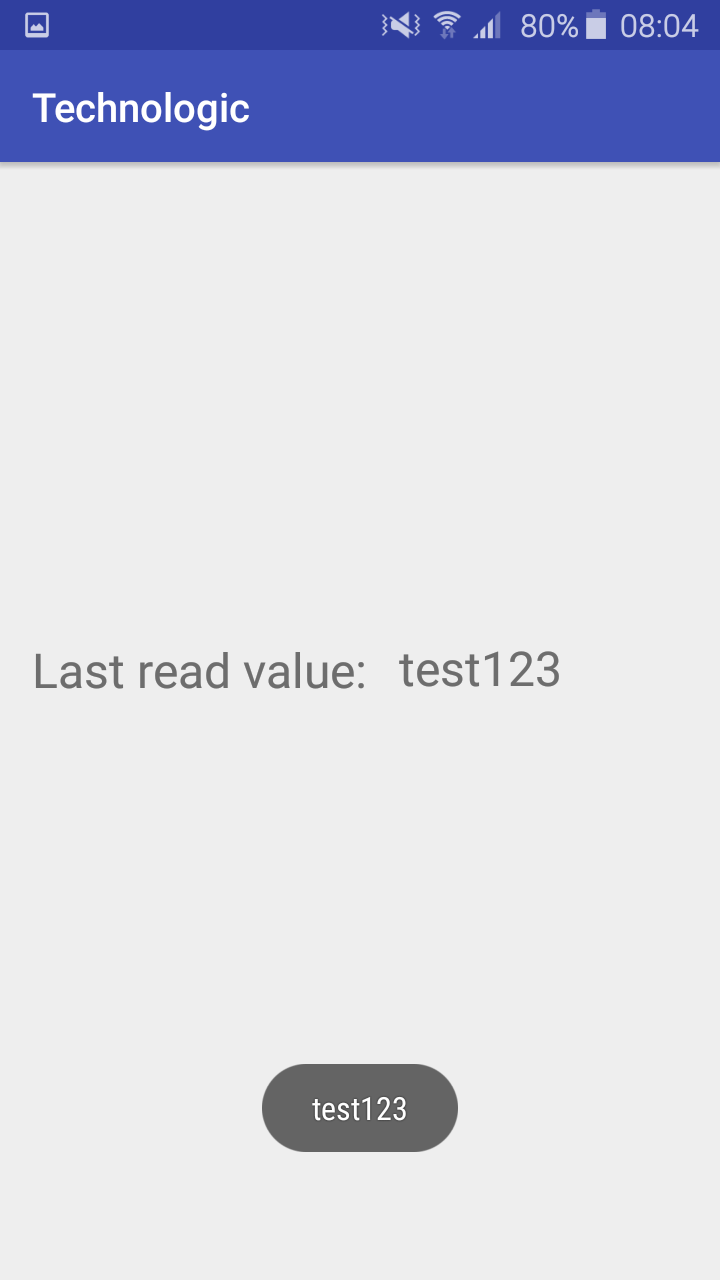
\includegraphics[scale=0.22]{imgs/read.png}
    \caption{Aktywność do odczytywania danych do tagu NFC}
\end{figure}
